%\VignetteIndexEntry{contextual: Simulating Contextual Multi-Armed Bandit Problems in R (article)}
%\VignetteEngine{knitr::knitr}
%\VignetteKeyword{archivsit}
%\VignetteKeyword{package}
%\VignetteKeyword{vignette}
%\VignetteKeyword{LaTeX}
\documentclass[nojss]{jss}\usepackage[]{graphicx}\usepackage[]{color}
%% maxwidth is the original width if it is less than linewidth
%% otherwise use linewidth (to make sure the graphics do not exceed the margin)
\makeatletter
\def\maxwidth{ %
  \ifdim\Gin@nat@width>\linewidth
    \linewidth
  \else
    \Gin@nat@width
  \fi
}
\makeatother

\definecolor{fgcolor}{rgb}{0.345, 0.345, 0.345}
\newcommand{\hlnum}[1]{\textcolor[rgb]{0.686,0.059,0.569}{#1}}%
\newcommand{\hlstr}[1]{\textcolor[rgb]{0.192,0.494,0.8}{#1}}%
\newcommand{\hlcom}[1]{\textcolor[rgb]{0.678,0.584,0.686}{\textit{#1}}}%
\newcommand{\hlopt}[1]{\textcolor[rgb]{0,0,0}{#1}}%
\newcommand{\hlstd}[1]{\textcolor[rgb]{0.345,0.345,0.345}{#1}}%
\newcommand{\hlkwa}[1]{\textcolor[rgb]{0.161,0.373,0.58}{\textbf{#1}}}%
\newcommand{\hlkwb}[1]{\textcolor[rgb]{0.69,0.353,0.396}{#1}}%
\newcommand{\hlkwc}[1]{\textcolor[rgb]{0.333,0.667,0.333}{#1}}%
\newcommand{\hlkwd}[1]{\textcolor[rgb]{0.737,0.353,0.396}{\textbf{#1}}}%
\let\hlipl\hlkwb

\usepackage{framed}
\makeatletter
\newenvironment{kframe}{%
 \def\at@end@of@kframe{}%
 \ifinner\ifhmode%
  \def\at@end@of@kframe{\end{minipage}}%
  \begin{minipage}{\columnwidth}%
 \fi\fi%
 \def\FrameCommand##1{\hskip\@totalleftmargin \hskip-\fboxsep
 \colorbox{shadecolor}{##1}\hskip-\fboxsep
     % There is no \\@totalrightmargin, so:
     \hskip-\linewidth \hskip-\@totalleftmargin \hskip\columnwidth}%
 \MakeFramed {\advance\hsize-\width
   \@totalleftmargin\z@ \linewidth\hsize
   \@setminipage}}%
 {\par\unskip\endMakeFramed%
 \at@end@of@kframe}
\makeatother

\definecolor{shadecolor}{rgb}{.97, .97, .97}
\definecolor{messagecolor}{rgb}{0, 0, 0}
\definecolor{warningcolor}{rgb}{1, 0, 1}
\definecolor{errorcolor}{rgb}{1, 0, 0}
\newenvironment{knitrout}{}{} % an empty environment to be redefined in TeX

\usepackage{alltt}

\usepackage[utf8]{inputenc}
\usepackage{color}

%% packages added by RvE
\usepackage{amssymb}
\usepackage{amsmath}
\usepackage{txfonts}
\usepackage{mathdots}
\usepackage{float}
\usepackage{algorithm}
\usepackage{algorithmic}
%\usepackage[classicReIm]{kpfonts}
%\usepackage[pdftex]{graphicx}

\DeclareMathOperator*{\argmax}{arg\,max}

\usepackage{natbib}
\usepackage[british]{babel} % for correct word hyphenation
\raggedbottom % for blank spaces at the bottom (e.g., references section)
%\setcounter{tocdepth}{3} % for table of contents
%\setcounter{secnumdepth}{3} % setting level of numbering
%%%%%%%%%%%%%%%%%%%%%%%%%%%%%%
%% declarations for jss.cls %%%%%%%%%%%%%%%%%%%%%%%%%%%%%%%%%%%%%%%%%%
%%%%%%%%%%%%%%%%%%%%%%%%%%%%%%

%% almost as usual
\author{Robin van Emden\\JADS \And
  Eric Postma\\Tilburg University \And
  Maurits Kaptein\\Tilburg University}

\title{\pkg{contextual}: Simulating Contextual Multi-Armed Bandit Problems in R}

%% for pretty printing and a nice hypersummary also set:
\Plainauthor{Robin van Emden, Eric Postma, Maurits Kaptein} %% comma-separated
\Plaintitle{contextual: Simulating Contextual Multi-Armed Bandit Problems in R} %% without formatting
\Shorttitle{\pkg{contextual}} %% a short title (if necessary)



%% an abstract and keywords
\Abstract{

Contextual multi-armed bandits have been gaining ever more popularity due to their effectiveness in solving previously computationally intractable partial information sequential decision problems - from online advertising and recommender systems to clinical trial design and personalized medicine. A popularity both inspired by and inspiring an ever-growing body of predominantly analytically oriented research on ever more sophisticated Contextual Bandit algorithms. At the same time, there are as of yet surprisingly few options that enable researchers and practitioners to simulate and compare the wealth of new and existing Bandit algorithms in a practical, standardized and extensible way. To help close this gap between analytical research and real-life application the current paper introduces the object-oriented R package \pkg{contextual}: a user-friendly and, though its clear object oriented structure, easily extensible framework that facilitates the comparison of, amongst others, contextual and non-contextual Bandit policies through both simulation and offline analysis. Furthermore, as the data generated in cMAB settings are often extremely large, much care has been taken to enable easy parallisation right out of the box.
}





\Keywords{contextual multi-armed bandits, simulation, sequential experimentation, \proglang{R}}
\Plainkeywords{contextual multi-armed bandits, simulation, sequential experimentation, R}

%% at least one keyword must be supplied

%% publication information
%% NOTE: Typically, this can be left commented and will be filled out by the technical editor
%% \Volume{50}
%% \Issue{9}
%% \Month{June}
%% \Year{2012}
%% \Submitdate{2012-06-04}
%% \Acceptdate{2012-06-04}

%% The address of (at least) one author should be given
%% in the following format:
\Address{
  Robin van Emden\\
  Jheronimus Academy of Data Science\\
  Den Bosch, the Netherlands\\
  E-mail: \email{robin@pwy.nl} \\
  URL: \url{pavlov.tech}\\
  \linebreak
  Eric O. Postma\\
  Tilburg University\\
  Communication and Information Sciences\\
  Tilburg, the Netherlands\\
  E-mail: \email{e.o.postma@tilburguniversity.edu}\\
  \linebreak
  Maurits C. Kaptein\\
  Tilburg University\\
  Statistics and Research Methods\\
  Tilburg, the Netherlands\\
  E-mail: \email{m.c.kaptein@uvt.nl}\\
  URL: \url{www.mauritskaptein.com}\\
}

%% It is also possible to add a telephone and fax number
%% before the e-mail in the following format:
%% Telephone: +43/512/507-7103
%% Fax: +43/512/507-2851

%% for those who use Sweave please include the following line (with % symbols):
%% need no \usepackage{Sweave.sty}

%% end of declarations %%%%%%%%%%%%%%%%%%%%%%%%%%%%%%%%%%%%%%%%%%%%%%%
\IfFileExists{upquote.sty}{\usepackage{upquote}}{}
\begin{document}

%% A vignette for the \cite{contextual} paper. #########################################RJKJLKJLKJDFDFSDFOIOPEIRPERE

%% include your article here, just as usual
%% Note that you should use the \pkg{}, \proglang{} and \code{} commands.




\section{Introduction}
%% Note: If there is markup in \(sub)section, then it has to be escape as above.

There are many real-world situations in which we repeatedly have to decide between a set of options, yet only learn about the best course of action by testing one choice after the other, one step at a time. Such problems are deceptively easy to state but have proven to have broad statistical and practical implications and applications. To get a better grip on such decision problems, and to learn why specific strategies might be more successful than others, they have been studied extensively under the title of \textquotedblleft{}Multi-Armed Bandit\textquotedblright{} problems. Here,  multi-armed bandits are defined as a statistical and machine learning concept in which a so-called agent follows the advice of an algorithm or \textquotedblleft{}policy\textquotedblright{} to optimize the overall reward it receives in a sequential decision problem with limited information. That is, a MAB policy suggests an agent when to explore new options and when to exploit known ones \textendash{} where, importantly, for each decision, at each time step t, the only new information the agent acquires is the reward for its latest decision. The agent remains in the dark about the potential rewards of the unchosen options and about any other information outside of current and past rewards and choices made.


In that respect, MAB problems reflect dilemmas we all encounter on a daily basis: do you stick to what you know and receive an expected result ("exploit") or choose something you don't know all that much about and potentially learn something new ("explore")?

\begin{itemize}
\item Do you feed your next coin to the one-armed bandit that paid out last time, or do you test your luck on another arm, on another machine?
\item When going out to dinner, do you explore new restaurants, or do you exploit familiar ones?
\item Do you stick to your current job, or explore and hunt around?
\item Do I keep my current stocks, or change my portfolio and pick some new ones?
\item As an online marketer, do you try a new ad, or keep the current one?
\item As a doctor, do you treat your patients with tried and tested medication, or do you prescribe a new and promising experimental treatment?
\end{itemize}

Though MAB models have already proven powerful of their own accord, a recent generalization, known as the \pkg{contextual} Multi-Armed Bandit (cMAB), adds one important element to the equation: in addition to past decisions and their rewards, cMAB agents are able to make use of side information about the state of the world at each t before making their decision. In other words, an agent that follows the advice of a cMAB policy may decide differently in different contexts.

This access to side information makes cMAB algorithms even more adept to many real-life decision problems than its MAB progenitors: do you show a certain add to returning customers, to new ones, or both? Do you prescribe a different treatment to male patients, female patients, or both? In the real world, it appears almost no choice exists without a context. So it may be no surprise that cMAB algorithms have found many applications: from recommender systems and advertising to health apps and personalized medicine. A practical applicability that has led to a multitude of new, often analytically derived bandit algorithms or policies, each with their own strengths and weaknesses.

Yet though cMAB algorithms have gained much traction in both research and industry, they have mostly been studied mathematically and analytically \textendash{} as of yet, comparisons on simulated, and, importantly, real-life large-scale offline \textquotedblleft{}partial label\textquotedblright{} data sets have been lacking. To this end, the current paper introduces the \pkg{contextual} R package. A package that aims to facilitate the simulation, offline comparison, and evaluation of (Contextual) Multi-Armed bandit policies. Though there exists one R package for basic MAB analysis, there is, as of yet, no extensible and widely applicable R package that is able to analyze and compare, respectively, basic K-armed, Continuum, Adversarial and Contextual Multi-Armed Bandit Algorithms on either simulated or online data.

In section 2, this paper will continue with a more formal definition of MAB and a CMAB problems and relate it to our implementation. In section 3, we will continue with an overview of \pkg{contextual}’s object oriented structure In section 4, we list the polices that are available by default, and simulate some MAB and a cMAB policy. In section 5, we demonstrate how easy it is to extend contextual with a policy (RVE: NOTE TO SELF: also custom  bandit?) of your own. In section 6, we replicate two papers, thereby demonstrating how to test policies on offline data sets. Finally, in section  7, we will go over some of the additional features in the package, and conclude with some comments on the current state of the package and possible enhancements.















\section{From formalisation to implementation}
%% Note: If there is markup in \(sub)section, then it has to be escape as above.

As stated above, a MAB problems can formaly stated with deceptive ease. First, state the number of arms \emph{k}, and the horizon, or number of rounds \emph{T}. Then, for each round \emph{t}= \{ 1, \ldots, T \}:

\begin{enumerate}
         \item[1)] An reward vector is generated \(r_{t}=\left( r_{1,t},  \dots, r_{k,t}\right)\)
         \item[2)] Agent A chooses an arm at \(a_{t} \in \left\{ 1, \dots, k \right\}\)
         \item[3)] Agent A receives a reward \(r_{a_{t},t}\)
\end{enumerate}

Where the goal of the agent is to miminize expected cumulative regret:

\begin{itemize}
         \item \( R_{T} = \mathbb{E}\left[ \textstyle \sum_{T}^{t=1}(r_{a*,t-r}) \right] = \mathbb{E}\left[ \textstyle \sum_{T}^{t=1}(\mu*-\mu_{a_{t}}) \right] \)
\end{itemize}

On implementing this basic formaliztion, the aforementioned sequential decision maker's exploit/explore dilemma can be captured by defining a finite set (or \textbf{bandit)} of \textit{K} i.i.d. options (the \textbf{arms }of the bandit\textbf{) }each with their own, unknown\textbf{, }reward distribution \textit{v${}_{1}$,{\dots},v${}_{k}$} with means \textit{$\mu$ {\dots} $\mu$${}_{k}$}. Next we define an \textbf{agent}, who has to decide between the exploration of unknown arms and the exploitation of known arms in \textit{K} in order to maximize its total\textbf{ reward} (that is, to maximize its cumulative reward $\sum_{t=1}^T r_t$ \footnote{or to minimize its cumulative or expected regret}) over a period of time $T$ by following the advice of a \textbf{policy $\boldsymbol{\piup}$} which keeps track of \textbf{parameters} \textbf{\textit{$\boldsymbol{\theta}$}}\textit{ }that are updated when new information (reward \textit{r} awarded by the bandit when the agent has chosen an arm) becomes available. This process is repeated \textit{T} times, where \textit{T} is often defined as the Bandit's "horizon".

In summary, an agent repeats the following lines one at a time at each time step \textit{t }in \textit{t}=1,2,{\dots},\textit{T}:

\begin{enumerate}
         \item[1a)] Agent asks policy $\piup$ which of the bandit's K arms to choose
         \item[1b)] Policy $\piup$ advices action \textit{a${}_{t}$} based on the state of a set of parameters \textit{$\theta$${}_{t}$}
         \item[2a)] Agent does action \textit{a${}_{t}$} by playing the suggested bandit arm.
         \item[2b)] Bandit rewards the agent with reward \textit{r${}_{t}$ }for action \textit{a${}_{t}$},
         \item[3a)] Agent sends the reward\textit{ r${}_{t}$ }to policy $\piup$
         \item[3b)] Policy $\piup$ uses \textit{r${}_{t}$} to update the policy's set of parameters\textit{ $\theta$${}_{t}$}
\end{enumerate}

\begin{figure}[H]
  \centering
    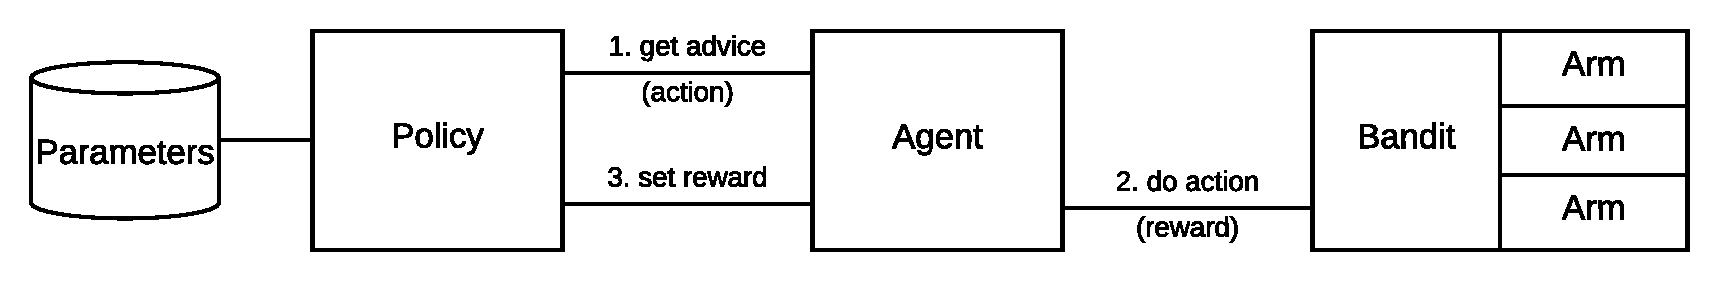
\includegraphics[width=.99\textwidth]{fig/mab_chart}
    \label{fig:mab_chart}
      \caption{Overview MAB formalization towards \pkg{contextual}'s implementation}
\end{figure}

To allow for side information, that is, to generalize this formalization to a \textit{contextual} Multi-Armed Bandit model, we need to state the number of feature \emph{d}, and add one first step to our model:

\begin{enumerate}
         \item[1)] A contextual feature vector is observed, \(x_{t}=\left( x_{1,t},  \dots, x_{d,t}\right)\)
         \item[2)] An reward vector is generated \(r_{t}=\left( r_{1,t},  \dots, r_{k,t}\right)\)
         \item[3)] Agent A chooses an arm at \(a_{t} \in \left\{ 1, \dots, k \right\}\)
         \item[4)] Agent A receives a reward \(r_{a_{t},t}\)
\end{enumerate}

From which follows that in our implementation, an agent repeats the following lines for each time step \textit{t} in \textit{t}=1,2,{\dots},\textit{T}:

\begin{enumerate}
         \item[1a)] Agent checks the bandit for side information that might influence the expression of its arms
         \item[1b)] Bandit returns feature vector \textit{Xt }
         \item[2a)] Agent asks policy $\piup$ which of the bandit's K arms to choose given \textit{Xt}
         \item[2b)] Given \textit{Xt}, policy $\piup$ advices action \textit{a${}_{t}$} based on the state of a set of parameters \textit{$\theta$${}_{t}$${}_{  }$}
         \item[3a)] Agent does action \textit{a${}_{t}$} by playing the suggested bandit arm.
         \item[3b)] Bandit rewards the agent with reward \textit{r${}_{t}$ }for action \textit{a${}_{t}$},
         \item[4a)] The agent sends the reward\textit{ r${}_{t}$ }to policy $\piup$
         \item[4b)] Policy $\piup$ uses \textit{r${}_{t}$} to update the policy's set of parameters\textit{ $\theta$${}_{t}$${}_{  }$}given \textit{Xt}
\end{enumerate}

\begin{figure}[H]
  \centering
    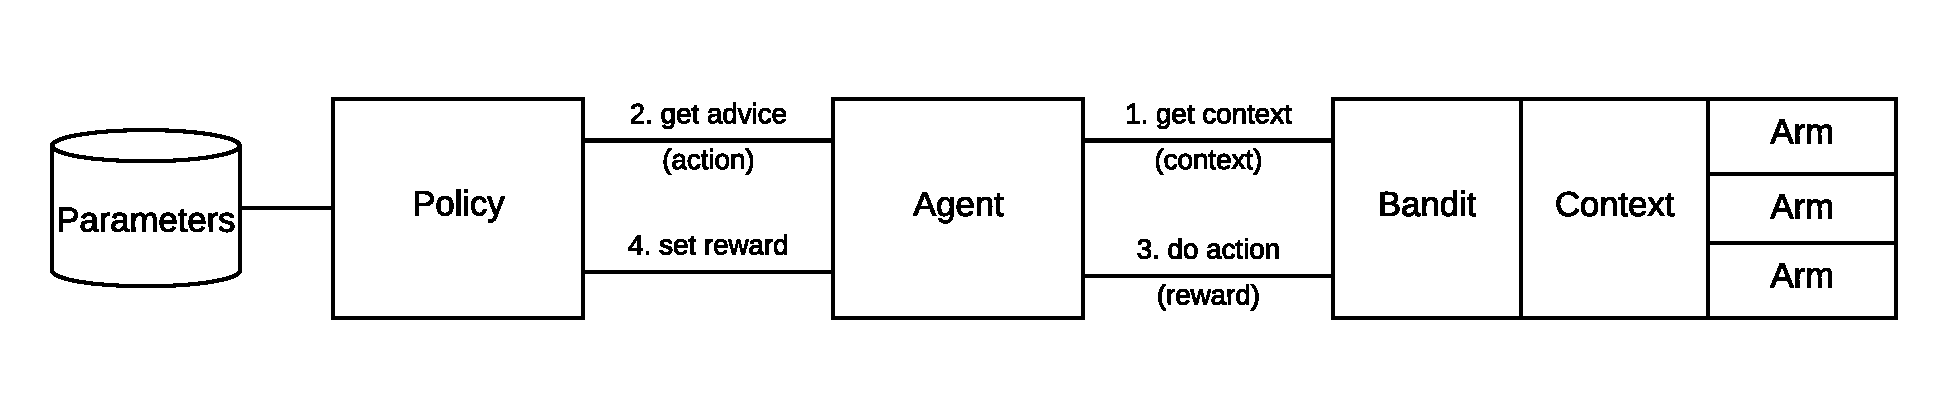
\includegraphics[width=.99\textwidth]{fig/cmab_chart}
    \label{fig:cmab_chart}
      \caption{Overview of cMAB formalization towards \pkg{contextual}'s implementation}
\end{figure}

As a matter of fact, when excluding a contextual feature, the suggested cMAB model perfectly emulates a non-contextual MAB model, easing the comparison and implementation of both MAB and cMAB substantially.











\section{Object-oriented setup of the package}
%% Note: If there is markup in \(sub)section, then it has to be escape as above.

Statistical computational methods, in R or otherwise,  are often made available through single-use scripts. Usually, these scripts are meant to give a basic idea of a statistical method, technique or algorithm in the context of a scientific paper. This is of no direct consequence within that particular setting. But when a set of well-researched interrelated algorithms find growing academic, practical and commercial adoption, it becomes crucial to offer a more standardized and more accessible way to compare different methods and algorithms.

A concern has become particularly pressing in the cMAB literature, where there is a tendency to publish analytical formalizations without any readily available script or implementation - while there is, at the same time, an ever growing interest in the practical application of cMAB algorithms.

The contextual package means to address this by making available an easily extendible framework, together with a library containing clear example implementations of several of the best known and most popular Contextual Bandit algorithms. For us, it made the most sense to create such a package in R. Firstly, as R is currently the de facto language for the dissemination of new statistical methods, techniques, and algorithms, while also being widely used in industry to simulate and test both new and existing algorithms. This makes it a sensible arena to bring together the interests, source code and data of both research and industry.

At the same time, it was clear to us that it would be of critical importance to make our R based framework as clear and as easily extensible as possible. We, therefore, chose to build our Object Oriented package on the R6 Object system. In contrast to the older S3 and S4 object systems, R6 methods are mutable and belong to their objects. That means that R6 objects behave, feel and look more like objects in computer languages like Python and Java. Together with its speed, simplicity, and clarity, we think contextual's use of R6 has indeed to enabled to achieve all of the aforemetioned goals.

The R6 package allows the creation of classes with reference semantics, similar to R's built-in reference classes. Yet compared to reference classes, R6 classes are simpler and lighter-weight, and they are not built on S4 classes, so they do not require the methods package. At the same time, classes do allow public and private members, and they support inheritance, even when the classes are defined in different packages. One R6 class can inherit from another. In other words, you can have super- and sub-classes. Subclasses can have additional methods, and they can also have methods that override the superclass methods.

This enabled us to translate the basic cMAB formalization from section 2 almost one on one to a clear object oriented structure. To clarify how our objects hang together, we created two UML diagrams. The UML class diagram shown in figure X visualizes the structure of our package by showcasing contextual's classes, attributes, and relationships between classes. The UML sequence diagram in figure X, on the other hand, shows how contextuals's classes behave over time. It depicts the objects and classes involved over one time step t, and it displays a basic version of the sequence of messages exchanged between all of contextual's basic objects.




\section{Basic use of the package}

Here, we show how to simulate some bandits, with their current implementation.

\subsection{Epsilon First}

In this algorithm, also known as AB(C) testing, a pure exploration phase is followed by a pure exploitation phase. The Epsilon First policy is equivalant to the setup of a randomized controlled trial (RCT): a study design where people are allocated at random to receive one of several clinical interventions. One of these interventions is the control. This control may be a standard practice, a placebo, or no intervention at all. On completion of the RCT, the best solution at that point is then suggested to be the superior "evidence based" option for everyone, at all times.

For figures, see Figure \ref{fig:fig1} on page \pageref{fig:fig1}.

The policy:

\begin{algorithm}
\caption{Epsilon First}
\label{Alg:EpsilonFirst}
\begin{algorithmic}
\REQUIRE \(   \eta \in \mathbb{Z}^{+} \)  , number of time steps $t$ in the exploration phase
\STATE \( n_{a} \leftarrow 0 \) for all arms a \(  \in \left\{ 1, \dots, k \right\} \)  (count how many times an arm has been chosen)
\STATE \( \hat{\mu}_{a} \leftarrow 0 \) for all arms a  \(   \in \left\{ 1, \dots, k \right\} \)  (estimate of expected reward per arm)
% Run through time points:
\FOR{$t=1, \dots, T$}
	% Run through arms. Step 1, select which one to play
	\IF {\(t \leq \eta\)}
	       \STATE play a random arm out of all arms a \(   \in \left\{ 1, \dots, k \right\} \)
	\ELSE
	        \STATE play arm \(a_t = \argmax_a  \hat{\mu}_{t=\eta,a}  \) with ties broken arbitrarily
	\ENDIF
	\STATE observe real-valued payoff $r_t$
	% Update:
	\STATE \( n_{a_{t}} \leftarrow n_{a_{t-1}} + 1  \)
   \STATE \( \hat{\mu}_{t,a_{t}} \leftarrow   \cfrac{r_t - \hat{\mu}_{t-1,a_{t}} }{n_{a_{t}}}   \)
\ENDFOR
\end{algorithmic}
\end{algorithm}


The EpsilonFirstPolicy class:

\begin{knitrout}\small
\definecolor{shadecolor}{rgb}{0.969, 0.969, 0.969}\color{fgcolor}\begin{kframe}
\begin{alltt}
\hlstd{EpsilonFirstPolicy} \hlkwb{<-} \hlstd{R6}\hlopt{::}\hlkwd{R6Class}\hlstd{(}
  \hlkwc{public} \hlstd{=} \hlkwd{list}\hlstd{(}
    \hlkwc{first} \hlstd{=} \hlkwa{NULL}\hlstd{,}
    \hlkwc{initialize} \hlstd{=} \hlkwa{function}\hlstd{(}\hlkwc{first} \hlstd{=} \hlnum{100}\hlstd{,} \hlkwc{name} \hlstd{=} \hlstr{"EpsilonFirst"}\hlstd{) \{}
      \hlstd{super}\hlopt{$}\hlkwd{initialize}\hlstd{(name)}
      \hlstd{self}\hlopt{$}\hlstd{first} \hlkwb{<-} \hlstd{first}
    \hlstd{\},}
    \hlkwc{set_parameters} \hlstd{=} \hlkwa{function}\hlstd{() \{}
      \hlstd{self}\hlopt{$}\hlstd{theta_to_arms} \hlkwb{<-} \hlkwd{list}\hlstd{(}\hlstr{'n'} \hlstd{=} \hlnum{0}\hlstd{,} \hlstr{'mean'} \hlstd{=} \hlnum{0}\hlstd{)}
    \hlstd{\},}
    \hlkwc{get_action} \hlstd{=} \hlkwa{function}\hlstd{(}\hlkwc{context}\hlstd{,} \hlkwc{t}\hlstd{) \{}
      \hlkwa{if} \hlstd{(}\hlkwd{sum_of}\hlstd{(theta}\hlopt{$}\hlstd{n)} \hlopt{<} \hlstd{first) \{}
        \hlstd{action}\hlopt{$}\hlstd{choice}          \hlkwb{<-} \hlkwd{sample.int}\hlstd{(context}\hlopt{$}\hlstd{k,} \hlnum{1}\hlstd{,} \hlkwc{replace} \hlstd{=} \hlnum{TRUE}\hlstd{)}
        \hlstd{action}\hlopt{$}\hlstd{propensity}   \hlkwb{<-} \hlstd{(}\hlnum{1}\hlopt{/}\hlstd{context}\hlopt{$}\hlstd{k)}
      \hlstd{\}} \hlkwa{else} \hlstd{\{}
        \hlstd{action}\hlopt{$}\hlstd{choice}          \hlkwb{<-} \hlkwd{max_in}\hlstd{(theta}\hlopt{$}\hlstd{mean,} \hlkwc{equal_is_random} \hlstd{=} \hlnum{FALSE}\hlstd{)}
        \hlstd{action}\hlopt{$}\hlstd{propensity}   \hlkwb{<-} \hlnum{1}
      \hlstd{\}}
      \hlstd{action}
    \hlstd{\},}
    \hlkwc{set_reward} \hlstd{=} \hlkwa{function}\hlstd{(}\hlkwc{context}\hlstd{,} \hlkwc{action}\hlstd{,} \hlkwc{reward}\hlstd{,} \hlkwc{t}\hlstd{) \{}
      \hlstd{arm}      \hlkwb{<-} \hlstd{action}\hlopt{$}\hlstd{choice}
      \hlstd{reward}   \hlkwb{<-} \hlstd{reward}\hlopt{$}\hlstd{reward}

      \hlkwd{inc}\hlstd{(theta}\hlopt{$}\hlstd{n[[arm]])} \hlkwb{<-} \hlnum{1}
      \hlkwa{if} \hlstd{(}\hlkwd{sum_of}\hlstd{(theta}\hlopt{$}\hlstd{n)} \hlopt{<} \hlstd{first} \hlopt{-} \hlnum{1}\hlstd{)}
        \hlkwd{inc}\hlstd{(theta}\hlopt{$}\hlstd{mean[[arm]] )} \hlkwb{<-} \hlstd{(reward} \hlopt{-} \hlstd{theta}\hlopt{$}\hlstd{mean[[arm]])} \hlopt{/} \hlstd{theta}\hlopt{$}\hlstd{n[[arm]]}

      \hlstd{theta}
    \hlstd{\}}
  \hlstd{)}
\hlstd{)}
\end{alltt}
\end{kframe}
\end{knitrout}

Running the policy:

\begin{knitrout}\small
\definecolor{shadecolor}{rgb}{0.969, 0.969, 0.969}\color{fgcolor}\begin{kframe}
\begin{alltt}
\hlkwd{library}\hlstd{(}\hlstr{"contextual"}\hlstd{)}

\hlstd{horizon}            \hlkwb{<-} \hlnum{100}
\hlstd{simulations}        \hlkwb{<-} \hlnum{100}
\hlstd{arm_weights}        \hlkwb{<-} \hlkwd{c}\hlstd{(}\hlnum{0.9}\hlstd{,} \hlnum{0.1}\hlstd{,} \hlnum{0.1}\hlstd{)}

\hlstd{policy}             \hlkwb{<-} \hlstd{EpsilonFirstPolicy}\hlopt{$}\hlkwd{new}\hlstd{(}\hlkwc{first} \hlstd{=} \hlnum{50}\hlstd{,} \hlkwc{name} \hlstd{=} \hlstr{"EFirst"}\hlstd{)}
\hlstd{bandit}             \hlkwb{<-} \hlstd{SyntheticBandit}\hlopt{$}\hlkwd{new}\hlstd{(}\hlkwc{arm_weights} \hlstd{= arm_weights)}

\hlstd{agent}              \hlkwb{<-} \hlstd{Agent}\hlopt{$}\hlkwd{new}\hlstd{(policy,bandit)}

\hlstd{simulator}          \hlkwb{<-} \hlstd{Simulator}\hlopt{$}\hlkwd{new}\hlstd{(}\hlkwc{agents} \hlstd{= agent,}
                                    \hlkwc{horizon} \hlstd{= horizon,}
                                    \hlkwc{simulations} \hlstd{= simulations)}

\hlstd{history}            \hlkwb{<-} \hlstd{simulator}\hlopt{$}\hlkwd{run}\hlstd{()}


\hlkwd{par}\hlstd{(}\hlkwc{mfrow} \hlstd{=} \hlkwd{c}\hlstd{(}\hlnum{1}\hlstd{,} \hlnum{2}\hlstd{),}\hlkwc{mar} \hlstd{=} \hlkwd{c}\hlstd{(}\hlnum{5}\hlstd{,} \hlnum{5}\hlstd{,} \hlnum{1}\hlstd{,} \hlnum{1}\hlstd{))}
\hlkwd{plot}\hlstd{(history,} \hlkwc{type} \hlstd{=} \hlstr{"cumulative"}\hlstd{)}
\hlkwd{plot}\hlstd{(history,} \hlkwc{type} \hlstd{=} \hlstr{"arms"}\hlstd{)}
\end{alltt}
\end{kframe}
\end{knitrout}

\begin{center}
\begin{knitrout}
\definecolor{shadecolor}{rgb}{0.969, 0.969, 0.969}\color{fgcolor}\begin{figure}[H]
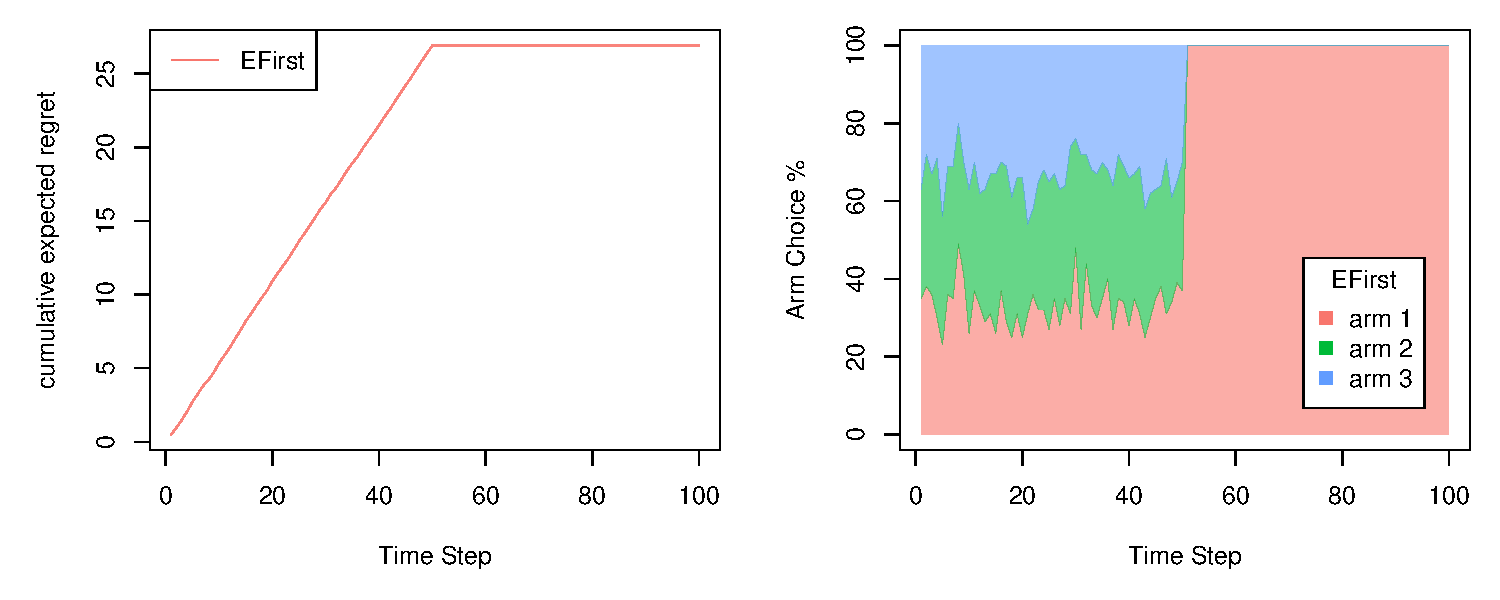
\includegraphics[width=\maxwidth,]{fig/fig1-1} \caption[Epsilon First]{Epsilon First}\label{fig:fig1}
\end{figure}


\end{knitrout}
\end{center}


\subsection{Epsilon Greedy}

This is an algorithm for continuously balancing exploration with exploitation. A randomly chosen arm is pulled a fraction $\epsilon$ of the time. The other 1-$\epsilon$ of the time, the arm with highest known payout is pulled.

For figures, see Figure \ref{fig:fig2} on page \pageref{fig:fig2}.

The algorithm:

\begin{algorithm}
\caption{Epsilon Greedy}
\label{Alg:EpsilonGreedy}
\begin{algorithmic}
\REQUIRE \(    \epsilon  \in \left[ 0,1 \right] \) - exploration tuning parameter
\STATE \( n_{a} \leftarrow 0 \) for all arms a \(  \in \left\{ 1, \dots, k \right\} \)  (count how many times an arm has been chosen)
\STATE \( \hat{\mu}_{a} \leftarrow 0 \) for all arms a  \(   \in \left\{ 1, \dots, k \right\} \)  (estimate of expected reward per arm)
% Run through time points:
\FOR{$t=1, \dots, T$}
	% Run through arms. Step 1, select which one to play
	\IF {sample from $\mathcal{N}(0,1) > \epsilon$}
		\STATE play arm \(a_t = \argmax_a  \hat{\mu}_{t-1,a}  \) with ties broken arbitrarily
	\ELSE
		\STATE play a random arm out of all arms a \(  \in \left\{ 1, \dots, k \right\} \)
	\ENDIF
	\STATE observe real-valued payoff $r_t$
	% Update:
	\STATE \( n_{a_{t}} \leftarrow n_{a_{t-1}} + 1  \)
   \STATE \( \hat{\mu}_{t,a_{t}} \leftarrow   \cfrac{r_t - \hat{\mu}_{t-1,a_{t}} }{n_{a_{t}}}   \)
\ENDFOR
\end{algorithmic}
\end{algorithm}

Translated to the EpsilonGreedyPolicy class:

\begin{knitrout}\small
\definecolor{shadecolor}{rgb}{0.969, 0.969, 0.969}\color{fgcolor}\begin{kframe}
\begin{alltt}
\hlstd{EpsilonGreedyPolicy} \hlkwb{<-} \hlstd{R6}\hlopt{::}\hlkwd{R6Class}\hlstd{(}
  \hlkwc{public} \hlstd{=} \hlkwd{list}\hlstd{(}
    \hlkwc{epsilon} \hlstd{=} \hlkwa{NULL}\hlstd{,}
    \hlkwc{initialize} \hlstd{=} \hlkwa{function}\hlstd{(}\hlkwc{epsilon} \hlstd{=} \hlnum{0.1}\hlstd{,} \hlkwc{name} \hlstd{=} \hlstr{"EGreedy"}\hlstd{) \{}
      \hlstd{super}\hlopt{$}\hlkwd{initialize}\hlstd{(name)}
      \hlstd{self}\hlopt{$}\hlstd{epsilon} \hlkwb{<-} \hlstd{epsilon}
    \hlstd{\},}
    \hlkwc{set_parameters} \hlstd{=} \hlkwa{function}\hlstd{() \{}
      \hlstd{self}\hlopt{$}\hlstd{theta_to_arms} \hlkwb{<-} \hlkwd{list}\hlstd{(}\hlstr{'n'} \hlstd{=} \hlnum{0}\hlstd{,} \hlstr{'mean'} \hlstd{=} \hlnum{0}\hlstd{)}
    \hlstd{\},}
    \hlkwc{get_action} \hlstd{=} \hlkwa{function}\hlstd{(}\hlkwc{context}\hlstd{,} \hlkwc{t}\hlstd{) \{}
      \hlkwa{if} \hlstd{(}\hlkwd{runif}\hlstd{(}\hlnum{1}\hlstd{)} \hlopt{>} \hlstd{epsilon) \{}
        \hlstd{action}\hlopt{$}\hlstd{choice} \hlkwb{<-} \hlkwd{max_in}\hlstd{(theta}\hlopt{$}\hlstd{mean)}
        \hlstd{action}\hlopt{$}\hlstd{propensity} \hlkwb{<-} \hlnum{1} \hlopt{-} \hlstd{self}\hlopt{$}\hlstd{epsilon}
      \hlstd{\}} \hlkwa{else} \hlstd{\{}
        \hlstd{action}\hlopt{$}\hlstd{choice} \hlkwb{<-} \hlkwd{sample.int}\hlstd{(context}\hlopt{$}\hlstd{k,} \hlnum{1}\hlstd{,} \hlkwc{replace} \hlstd{=} \hlnum{TRUE}\hlstd{)}
        \hlstd{action}\hlopt{$}\hlstd{propensity} \hlkwb{<-} \hlstd{epsilon}\hlopt{*}\hlstd{(}\hlnum{1}\hlopt{/}\hlstd{context}\hlopt{$}\hlstd{k)}
      \hlstd{\}}
      \hlstd{action}
    \hlstd{\},}
    \hlkwc{set_reward} \hlstd{=} \hlkwa{function}\hlstd{(}\hlkwc{context}\hlstd{,} \hlkwc{action}\hlstd{,} \hlkwc{reward}\hlstd{,} \hlkwc{t}\hlstd{) \{}
      \hlstd{arm} \hlkwb{<-} \hlstd{action}\hlopt{$}\hlstd{choice}
      \hlstd{reward} \hlkwb{<-} \hlstd{reward}\hlopt{$}\hlstd{reward}
      \hlkwd{inc}\hlstd{(theta}\hlopt{$}\hlstd{n[[arm]])}    \hlkwb{<-} \hlnum{1}
      \hlkwd{inc}\hlstd{(theta}\hlopt{$}\hlstd{mean[[arm]])} \hlkwb{<-} \hlstd{(reward} \hlopt{-} \hlstd{theta}\hlopt{$}\hlstd{mean[[arm]])} \hlopt{/} \hlstd{theta}\hlopt{$}\hlstd{n[[arm]]}
      \hlstd{theta}
    \hlstd{\}}
  \hlstd{)}
\hlstd{)}
\end{alltt}
\end{kframe}
\end{knitrout}

How to run it:

\begin{knitrout}\small
\definecolor{shadecolor}{rgb}{0.969, 0.969, 0.969}\color{fgcolor}\begin{kframe}
\begin{alltt}
\hlkwd{library}\hlstd{(}\hlstr{"contextual"}\hlstd{)}

\hlstd{horizon}            \hlkwb{<-} \hlnum{100}
\hlstd{simulations}        \hlkwb{<-} \hlnum{100}
\hlstd{arm_weights}        \hlkwb{<-} \hlkwd{c}\hlstd{(}\hlnum{0.9}\hlstd{,} \hlnum{0.1}\hlstd{,} \hlnum{0.1}\hlstd{)}

\hlstd{policy}             \hlkwb{<-} \hlstd{EpsilonGreedyPolicy}\hlopt{$}\hlkwd{new}\hlstd{(}\hlkwc{epsilon} \hlstd{=} \hlnum{0.1}\hlstd{,} \hlkwc{name} \hlstd{=} \hlstr{"EG"}\hlstd{)}
\hlstd{bandit}             \hlkwb{<-} \hlstd{SyntheticBandit}\hlopt{$}\hlkwd{new}\hlstd{(}\hlkwc{arm_weights} \hlstd{= arm_weights)}

\hlstd{agent}              \hlkwb{<-} \hlstd{Agent}\hlopt{$}\hlkwd{new}\hlstd{(policy,bandit)}

\hlstd{simulator}          \hlkwb{<-} \hlstd{Simulator}\hlopt{$}\hlkwd{new}\hlstd{(}\hlkwc{agents} \hlstd{= agent,}
                                    \hlkwc{horizon} \hlstd{= horizon,}
                                    \hlkwc{simulations} \hlstd{= simulations)}

\hlstd{history}            \hlkwb{<-} \hlstd{simulator}\hlopt{$}\hlkwd{run}\hlstd{()}


\hlkwd{par}\hlstd{(}\hlkwc{mfrow} \hlstd{=} \hlkwd{c}\hlstd{(}\hlnum{1}\hlstd{,} \hlnum{2}\hlstd{),}\hlkwc{mar} \hlstd{=} \hlkwd{c}\hlstd{(}\hlnum{5}\hlstd{,} \hlnum{5}\hlstd{,} \hlnum{1}\hlstd{,} \hlnum{1}\hlstd{))}
\hlkwd{plot}\hlstd{(history,} \hlkwc{type} \hlstd{=} \hlstr{"cumulative"}\hlstd{)}
\hlkwd{plot}\hlstd{(history,} \hlkwc{type} \hlstd{=} \hlstr{"arms"}\hlstd{)}
\end{alltt}
\end{kframe}
\end{knitrout}

\begin{center}
\begin{knitrout}
\definecolor{shadecolor}{rgb}{0.969, 0.969, 0.969}\color{fgcolor}\begin{figure}[H]
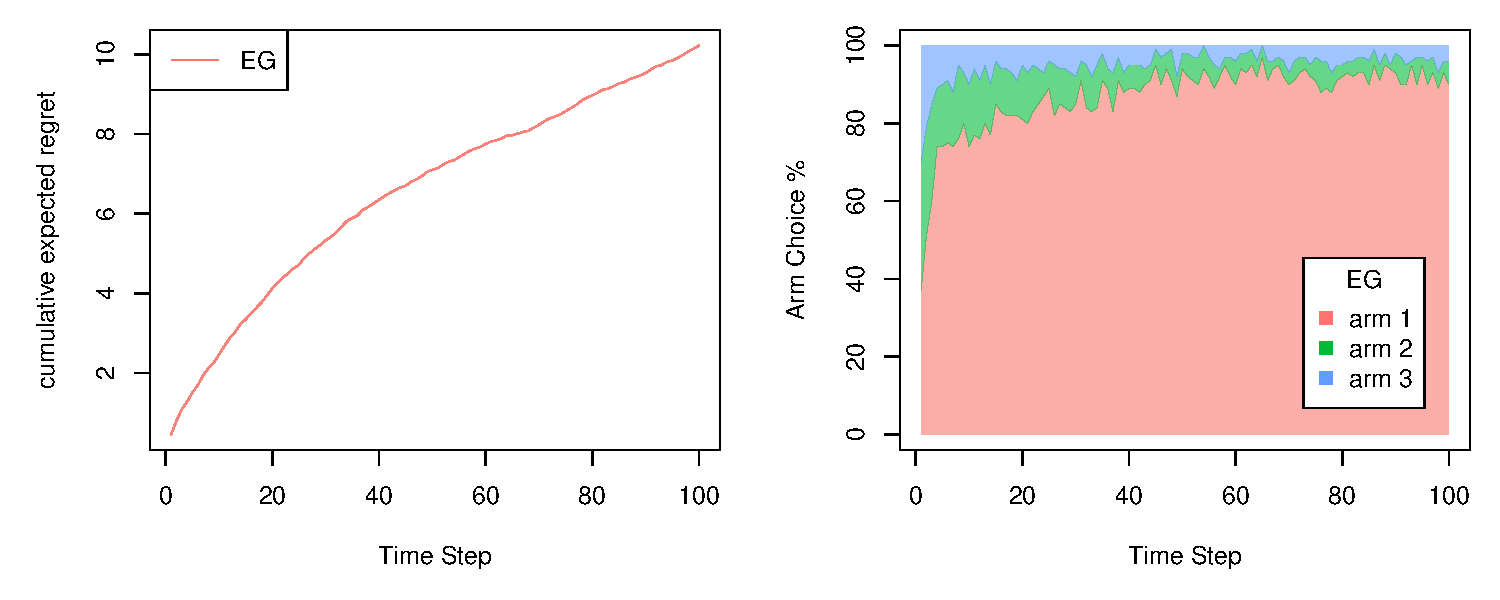
\includegraphics[width=\maxwidth,]{fig/fig2-1} \caption[Epsilon Greedy]{Epsilon Greedy}\label{fig:fig2}
\end{figure}


\end{knitrout}
\end{center}

\subsection{Contextual Bandit: LinUCB with Linear Disjoint Models}

The algorithm:

\begin{algorithm}
\caption{LinUCB with linear disjoint models}
\label{Alg:LinUCBDisjoint}
\begin{algorithmic}
\REQUIRE $\alpha$ \(  \in \mathbb{R}^{+} \), exploration tuning parameter
% Run through time points:
\FOR{$t=1, \dots, T$}
          \STATE Observe features of all arms \(  a \in \mathcal{A}_{t}: x_{t,a} \in \mathbb{R}^{d}\)
	% Run through arms. Step 1, select which one to play
	\FOR{ \(  a \in \mathcal{A}_{t}\)}
	          \IF{\(a\) is new}
		      \STATE \(A_{a} \leftarrow I_{d}  \)  (d-dimensional identity matrix)
		      \STATE \(b_{a} \leftarrow 0_{d\times1}   \) (d-dimensional zero vector)
		\ENDIF
		\STATE \( \hat{\theta}_{a} \leftarrow A_{a}^{-1}b_{a} \)
		\STATE \( p_{t,a} \leftarrow \hat{\theta}_{a}^{T} + \alpha  \sqrt{ x_{t,a}^{T} A_{a}^{-1}x_{t,a}} \)
	\ENDFOR
	% allocate to arm
	\STATE Play arm \(a_t = \argmax_a  p_{t,a}  \) with ties broken arbitrarily and observe real-valued payoff $r_t$
	% Update:
           \STATE \( A_{a_{t}} \leftarrow A_{a_{t}}+ x_{t,a_{t}}x_{t,a_{t}}^{T} \)
           \STATE  \( b_{a_{t}} \leftarrow b_{a_{t}}+ r_{t}x_{t,a_{t}}  \)
\ENDFOR
\end{algorithmic}
\end{algorithm}

This is how the algorithm works: at each step, we run a linear regression with the data we have collected so far such that we have a coefficient for each context feature. We then observe our new context, and generate a predicted payoff using our model. We also generate a confidence interval for that predicted payoff for each of the three arms. We then choose the arm with the highest upper confidence bound.

For figures, see Figure \ref{fig:fig3} on page \pageref{fig:fig3}.

\begin{knitrout}\small
\definecolor{shadecolor}{rgb}{0.969, 0.969, 0.969}\color{fgcolor}\begin{kframe}
\begin{alltt}
\hlcom{#' @export}
\hlstd{LinUCBDisjointPolicy} \hlkwb{<-} \hlstd{R6}\hlopt{::}\hlkwd{R6Class}\hlstd{(}
  \hlkwc{public} \hlstd{=} \hlkwd{list}\hlstd{(}
    \hlkwc{alpha} \hlstd{=} \hlkwa{NULL}\hlstd{,}
    \hlkwc{initialize} \hlstd{=} \hlkwa{function}\hlstd{(}\hlkwc{alpha} \hlstd{=} \hlnum{1.0}\hlstd{,} \hlkwc{name} \hlstd{=} \hlstr{"LinUCBDisjoint"}\hlstd{) \{}
      \hlstd{super}\hlopt{$}\hlkwd{initialize}\hlstd{(name)}
      \hlstd{self}\hlopt{$}\hlstd{alpha} \hlkwb{<-} \hlstd{alpha}
    \hlstd{\},}
    \hlkwc{set_parameters} \hlstd{=} \hlkwa{function}\hlstd{() \{}
      \hlstd{self}\hlopt{$}\hlstd{theta_to_arms} \hlkwb{<-} \hlkwd{list}\hlstd{(} \hlstr{'A'} \hlstd{=} \hlkwd{diag}\hlstd{(}\hlnum{1}\hlstd{,self}\hlopt{$}\hlstd{d,self}\hlopt{$}\hlstd{d),} \hlstr{'b'} \hlstd{=} \hlkwd{rep}\hlstd{(}\hlnum{0}\hlstd{,self}\hlopt{$}\hlstd{d))}
    \hlstd{\},}
    \hlkwc{get_action} \hlstd{=} \hlkwa{function}\hlstd{(}\hlkwc{context}\hlstd{,} \hlkwc{t}\hlstd{) \{}
      \hlstd{expected_rewards} \hlkwb{<-} \hlkwd{rep}\hlstd{(}\hlnum{0.0}\hlstd{, context}\hlopt{$}\hlstd{k)}
      \hlkwa{for} \hlstd{(arm} \hlkwa{in} \hlnum{1}\hlopt{:}\hlstd{self}\hlopt{$}\hlstd{k) \{}
        \hlstd{X}          \hlkwb{<-}  \hlstd{context}\hlopt{$}\hlstd{X[,arm]}
        \hlstd{A}          \hlkwb{<-}  \hlstd{theta}\hlopt{$}\hlstd{A[[arm]]}
        \hlstd{b}          \hlkwb{<-}  \hlstd{theta}\hlopt{$}\hlstd{b[[arm]]}
        \hlstd{A_inv}      \hlkwb{<-}  \hlkwd{solve}\hlstd{(A)}

        \hlstd{theta_hat}  \hlkwb{<-}  \hlstd{A_inv} \hlopt \hlstd{b}
        \hlstd{mean}       \hlkwb{<-}  \hlstd{X} \hlopt \hlstd{theta_hat}
        \hlstd{sd}         \hlkwb{<-}  \hlkwd{sqrt}\hlstd{(}\hlkwd{tcrossprod}\hlstd{(X} \hlopt \hlstd{A_inv, X))}
        \hlstd{expected_rewards[arm]} \hlkwb{<-} \hlstd{mean} \hlopt{+} \hlstd{alpha} \hlopt{*} \hlstd{sd}
      \hlstd{\}}
      \hlstd{action}\hlopt{$}\hlstd{choice}  \hlkwb{<-} \hlkwd{max_in}\hlstd{(expected_rewards)}
      \hlstd{action}
    \hlstd{\},}
    \hlkwc{set_reward} \hlstd{=} \hlkwa{function}\hlstd{(}\hlkwc{context}\hlstd{,} \hlkwc{action}\hlstd{,} \hlkwc{reward}\hlstd{,} \hlkwc{t}\hlstd{) \{}
      \hlstd{arm} \hlkwb{<-} \hlstd{action}\hlopt{$}\hlstd{choice}
      \hlstd{reward} \hlkwb{<-} \hlstd{reward}\hlopt{$}\hlstd{reward}
      \hlstd{Xa} \hlkwb{<-} \hlstd{context}\hlopt{$}\hlstd{X[,arm]}

      \hlkwd{inc}\hlstd{(theta}\hlopt{$}\hlstd{A[[arm]])} \hlkwb{<-} \hlkwd{outer}\hlstd{(Xa, Xa)}
      \hlkwd{inc}\hlstd{(theta}\hlopt{$}\hlstd{b[[arm]])} \hlkwb{<-} \hlstd{reward} \hlopt{*} \hlstd{Xa}

      \hlstd{theta}
    \hlstd{\}}
  \hlstd{)}
\hlstd{)}
\end{alltt}
\end{kframe}
\end{knitrout}


\begin{knitrout}\small
\definecolor{shadecolor}{rgb}{0.969, 0.969, 0.969}\color{fgcolor}\begin{kframe}
\begin{alltt}
\hlstd{horizon}          \hlkwb{<-} \hlnum{100L}
\hlstd{simulations}      \hlkwb{<-} \hlnum{300L}
                              \hlcom{# k=1  k=2  k=3           columns represent arms}
\hlstd{context_weights}  \hlkwb{<-} \hlkwd{matrix}\hlstd{(}  \hlkwd{c}\hlstd{(} \hlnum{0.9}\hlstd{,} \hlnum{0.1}\hlstd{,} \hlnum{0.1}\hlstd{,}  \hlcom{# d=1}
                                \hlnum{0.1}\hlstd{,} \hlnum{0.9}\hlstd{,} \hlnum{0.1}\hlstd{,}  \hlcom{# d=2}
                                \hlnum{0.1}\hlstd{,} \hlnum{0.1}\hlstd{,} \hlnum{0.9}\hlstd{),} \hlcom{# d=3   rows for context features}

                                \hlkwc{nrow} \hlstd{=} \hlnum{3}\hlstd{,} \hlkwc{ncol} \hlstd{=} \hlnum{3}\hlstd{,} \hlkwc{byrow} \hlstd{=} \hlnum{TRUE}\hlstd{)}

\hlstd{bandit}           \hlkwb{<-} \hlstd{SyntheticBandit}\hlopt{$}\hlkwd{new}\hlstd{(}\hlkwc{context_weights} \hlstd{= context_weights)}

\hlstd{agents}           \hlkwb{<-} \hlkwd{list}\hlstd{(Agent}\hlopt{$}\hlkwd{new}\hlstd{(EpsilonGreedyPolicy}\hlopt{$}\hlkwd{new}\hlstd{(}\hlnum{0.1}\hlstd{,} \hlstr{"Egreedy"}\hlstd{), bandit),}
                         \hlstd{Agent}\hlopt{$}\hlkwd{new}\hlstd{(OraclePolicy}\hlopt{$}\hlkwd{new}\hlstd{(}\hlstr{"Oracle"}\hlstd{), bandit),}
                         \hlstd{Agent}\hlopt{$}\hlkwd{new}\hlstd{(LinUCBDisjointPolicy}\hlopt{$}\hlkwd{new}\hlstd{(}\hlnum{1.0}\hlstd{,} \hlstr{"LinUCB"}\hlstd{), bandit))}

\hlstd{simulation}       \hlkwb{<-} \hlstd{Simulator}\hlopt{$}\hlkwd{new}\hlstd{(agents, horizon, simulations)}
\hlstd{history}          \hlkwb{<-} \hlstd{simulation}\hlopt{$}\hlkwd{run}\hlstd{()}

\hlkwd{par}\hlstd{(}\hlkwc{mfrow} \hlstd{=} \hlkwd{c}\hlstd{(}\hlnum{1}\hlstd{,} \hlnum{2}\hlstd{),}\hlkwc{mar} \hlstd{=} \hlkwd{c}\hlstd{(}\hlnum{5}\hlstd{,} \hlnum{5}\hlstd{,} \hlnum{1}\hlstd{,} \hlnum{1}\hlstd{))}
\hlkwd{plot}\hlstd{(history,} \hlkwc{type} \hlstd{=} \hlstr{"cumulative"}\hlstd{)}
\hlkwd{plot}\hlstd{(history,} \hlkwc{type} \hlstd{=} \hlstr{"cumulative"}\hlstd{,} \hlkwc{regret} \hlstd{=} \hlnum{FALSE}\hlstd{)}
\end{alltt}
\end{kframe}
\end{knitrout}

\begin{center}
\begin{knitrout}
\definecolor{shadecolor}{rgb}{0.969, 0.969, 0.969}\color{fgcolor}\begin{figure}[H]
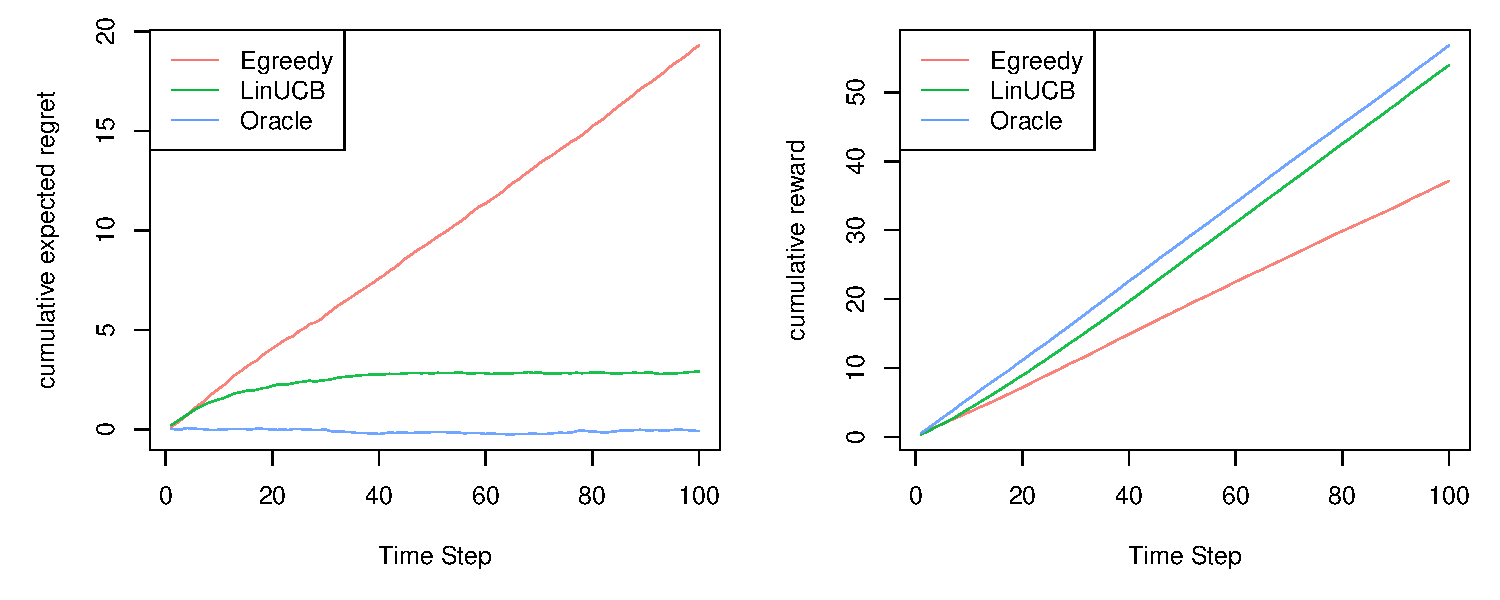
\includegraphics[width=\maxwidth,]{fig/fig3-1} \caption[LinUCB algorithm with linear disjoint models, following Li et al]{LinUCB algorithm with linear disjoint models, following Li et al. (2010)}\label{fig:fig3}
\end{figure}


\end{knitrout}
\end{center}

\section{Extending the package}

Through its R6 based object system, it's relatively easy to extend contextual. Below, we demonstrate how to make use of that extensibility through the implementation of a PoissonRewardBandit extending contextual's BasicBandit class, and of an PoissonRewardBandit version of the Epsilon Greedy policy presented above.

\begin{knitrout}\small
\definecolor{shadecolor}{rgb}{0.969, 0.969, 0.969}\color{fgcolor}\begin{kframe}
\begin{alltt}
\hlstd{PoissonRewardBandit} \hlkwb{<-} \hlstd{R6}\hlopt{::}\hlkwd{R6Class}\hlstd{(}
  \hlstr{"PoissonRewardBandit"}\hlstd{,}
  \hlcom{# Class extends BasicBandit}
  \hlkwc{inherit} \hlstd{= BasicBandit,}
  \hlkwc{public} \hlstd{=} \hlkwd{list}\hlstd{(}
    \hlkwc{initialize}   \hlstd{=} \hlkwa{function}\hlstd{(}\hlkwc{weights}\hlstd{) \{}
      \hlstd{super}\hlopt{$}\hlkwd{initialize}\hlstd{(weights)}
    \hlstd{\},}
    \hlcom{# Overrides BasicBandit's do_action to generate Poisson based rewards}
    \hlkwc{do_action} \hlstd{=} \hlkwa{function}\hlstd{(}\hlkwc{action}\hlstd{,} \hlkwc{t}\hlstd{) \{}
      \hlstd{reward_means} \hlkwb{=} \hlkwd{c}\hlstd{(}\hlnum{2}\hlstd{,}\hlnum{2}\hlstd{,}\hlnum{2}\hlstd{)}
      \hlstd{private}\hlopt{$}\hlstd{R} \hlkwb{<-} \hlkwd{matrix}\hlstd{(}\hlkwd{rpois}\hlstd{(}\hlnum{3}\hlstd{, reward_means)} \hlopt{<} \hlstd{self}\hlopt{$}\hlkwd{get_weights}\hlstd{(), self}\hlopt{$}\hlstd{k, self}\hlopt{$}\hlstd{d)}\hlopt{*}\hlnum{1}
      \hlstd{private}\hlopt{$}\hlkwd{reward_to_list}\hlstd{(action, t)}
    \hlstd{\}}
  \hlstd{)}
\hlstd{)}

\hlstd{EpsilonGreedyAnnealingPolicy} \hlkwb{<-} \hlstd{R6}\hlopt{::}\hlkwd{R6Class}\hlstd{(}
  \hlstr{"EpsilonGreedyAnnealingPolicy"}\hlstd{,}
  \hlcom{# Class extends EpsilonGreedyPolicy}
  \hlkwc{inherit} \hlstd{= EpsilonGreedyPolicy,}
  \hlkwc{portable} \hlstd{=} \hlnum{FALSE}\hlstd{,}
  \hlkwc{class} \hlstd{=} \hlnum{FALSE}\hlstd{,}
  \hlkwc{public} \hlstd{=} \hlkwd{list}\hlstd{(}
    \hlkwc{get_action} \hlstd{=} \hlkwa{function}\hlstd{(}\hlkwc{context}\hlstd{,} \hlkwc{t}\hlstd{) \{}
      \hlcom{# Override get_action to make annealing}
      \hlstd{epsilon} \hlkwb{=} \hlnum{1} \hlopt{/} \hlkwd{log}\hlstd{(t} \hlopt{+} \hlnum{0.0000001}\hlstd{)}
      \hlkwa{if} \hlstd{(}\hlkwd{runif}\hlstd{(}\hlnum{1}\hlstd{)} \hlopt{>} \hlstd{epsilon) \{}
        \hlstd{action}\hlopt{$}\hlstd{choice} \hlkwb{<-} \hlkwd{max_in}\hlstd{(theta}\hlopt{$}\hlstd{mean)}
        \hlstd{action}\hlopt{$}\hlstd{propensity} \hlkwb{<-} \hlnum{1} \hlopt{-} \hlstd{self}\hlopt{$}\hlstd{epsilon}
      \hlstd{\}} \hlkwa{else} \hlstd{\{}
        \hlstd{action}\hlopt{$}\hlstd{choice} \hlkwb{<-} \hlkwd{sample.int}\hlstd{(context}\hlopt{$}\hlstd{k,} \hlnum{1}\hlstd{,} \hlkwc{replace} \hlstd{=} \hlnum{TRUE}\hlstd{)}
        \hlstd{action}\hlopt{$}\hlstd{propensity} \hlkwb{<-} \hlstd{epsilon}\hlopt{*}\hlstd{(}\hlnum{1}\hlopt{/}\hlstd{context}\hlopt{$}\hlstd{k)}
      \hlstd{\}}
      \hlstd{action}
    \hlstd{\}}
  \hlstd{)}
\hlstd{)}

\hlstd{weights}     \hlkwb{<-} \hlkwd{c}\hlstd{(}\hlnum{7}\hlstd{,}\hlnum{1}\hlstd{,}\hlnum{2}\hlstd{)}
\hlstd{bandit}      \hlkwb{<-} \hlstd{PoissonRewardBandit}\hlopt{$}\hlkwd{new}\hlstd{(weights)}
\hlstd{agents}      \hlkwb{<-} \hlkwd{list}\hlstd{( Agent}\hlopt{$}\hlkwd{new}\hlstd{(EpsilonGreedyPolicy}\hlopt{$}\hlkwd{new}\hlstd{(}\hlnum{0.1}\hlstd{,} \hlstr{"EG Annealing"}\hlstd{), bandit),}
                     \hlstd{Agent}\hlopt{$}\hlkwd{new}\hlstd{(EpsilonGreedyAnnealingPolicy}\hlopt{$}\hlkwd{new}\hlstd{(}\hlnum{0.1}\hlstd{,} \hlstr{"EG"}\hlstd{), bandit) )}
\hlstd{simulation}  \hlkwb{<-} \hlstd{Simulator}\hlopt{$}\hlkwd{new}\hlstd{(agents,} \hlkwc{horizon} \hlstd{=} \hlnum{200L}\hlstd{,} \hlkwc{simulations} \hlstd{=} \hlnum{100L}\hlstd{)}

\hlstd{history}     \hlkwb{<-} \hlstd{simulation}\hlopt{$}\hlkwd{run}\hlstd{()}

\hlkwd{par}\hlstd{(}\hlkwc{mfrow} \hlstd{=} \hlkwd{c}\hlstd{(}\hlnum{1}\hlstd{,} \hlnum{2}\hlstd{),}\hlkwc{mar} \hlstd{=} \hlkwd{c}\hlstd{(}\hlnum{5}\hlstd{,} \hlnum{5}\hlstd{,} \hlnum{1}\hlstd{,} \hlnum{1}\hlstd{))}
\hlkwd{plot}\hlstd{(history,} \hlkwc{type} \hlstd{=} \hlstr{"cumulative"}\hlstd{)}
\hlkwd{plot}\hlstd{(history,} \hlkwc{type} \hlstd{=} \hlstr{"average"}\hlstd{,} \hlkwc{regret} \hlstd{=} \hlnum{FALSE}\hlstd{)}
\end{alltt}
\end{kframe}
\end{knitrout}

\begin{center}
\begin{knitrout}
\definecolor{shadecolor}{rgb}{0.969, 0.969, 0.969}\color{fgcolor}\begin{figure}[H]
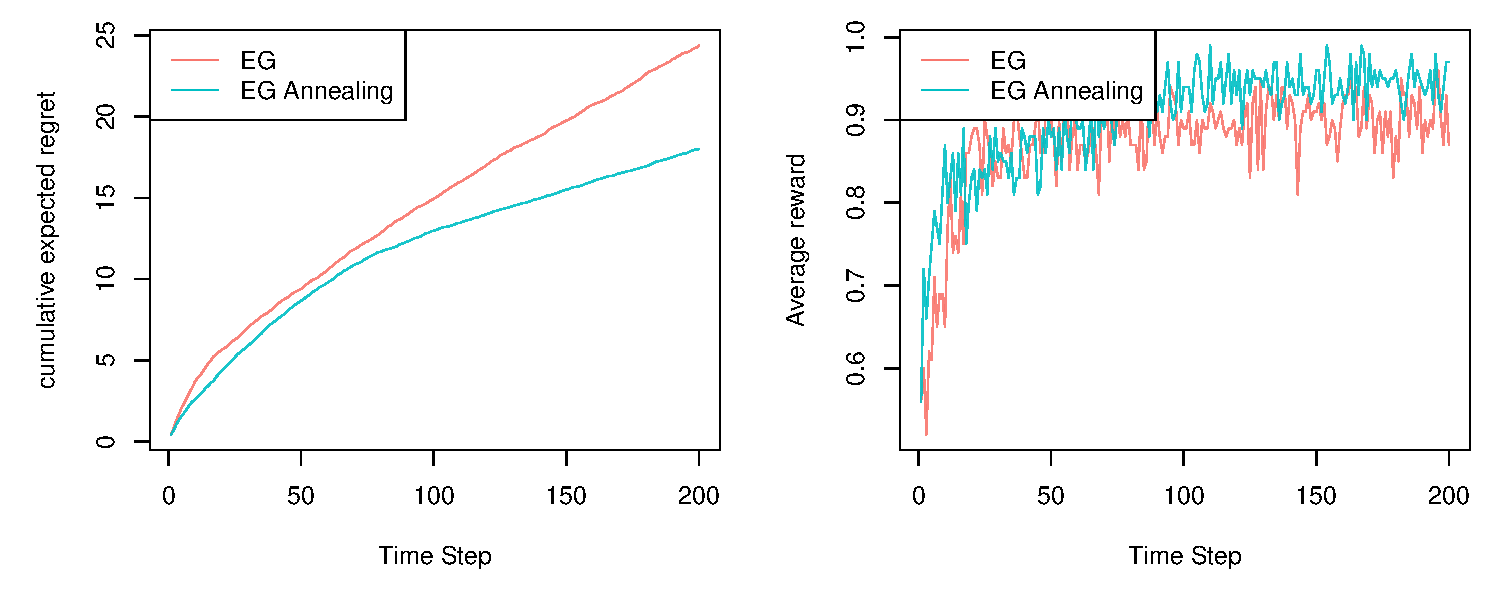
\includegraphics[width=\maxwidth,]{fig/fig4-1} \caption[Extending BasicBandit and EpsilonGreedyPolicy]{Extending BasicBandit and EpsilonGreedyPolicy}\label{fig:fig4}
\end{figure}


\end{knitrout}
\end{center}


\section{Simulation and Offline evaluation Bandits}

\subsection{Simulation}

Some info on the implemented simulating Bandits, inc strengths and weakenesses.

*** Basic very simple ***

*** Based on modeling ***

\subsection{Offline evaluation}

\subsubsection{Offline evaluation through LiLogBandit}

Though it is, as demonstrated in the previous section, relatively easy to create basic simulators to test simple MAB and cMAB policies, the creation of more complex simulations that generate more complex contexts for more demanding policies can become very complicated very fast. So much so, that the implementation of such simulators regularly becomes more complex than the analysis and implementation of the policies themselves. More seriously, even when succeeding in surpassing these technical challenges, it remains an open question if an evaluation based on simulated data reflects real-world applications, as modeling by definition introduces bias.

But there exists another, unbiased approach to testing MAB and cMAB policies. This approach makes use of widely available offline sources of data and can pre-empt the issues of bias and model complexity. It also offers the secondary advantages that offline data is both widely available and reflective of real-world online interactions. But there is one catch, that is particular to the evaluation of MAB problems: when we seek to make use of offline data, we miss out on user feedback when a policy advices a different arm than the one the user selected. In other words, offline data is only "partially labeled" with respect to any Bandit policies, as bandit evaluations only contain user feedback for arms that were displayed to the agent but include no information on other arms.

*** explain how li log algorithm helps here***

*** insert algorithm ***


*** insert code ***


\subsubsection{Offline evaluation through DoublyRobustBandit}



*** insert algorithm ***


*** insert code ***

\section{Replications with offline data}

Here we replicate some papers with a huge offline dataset..

\begin{figure}[H]
  \centering
    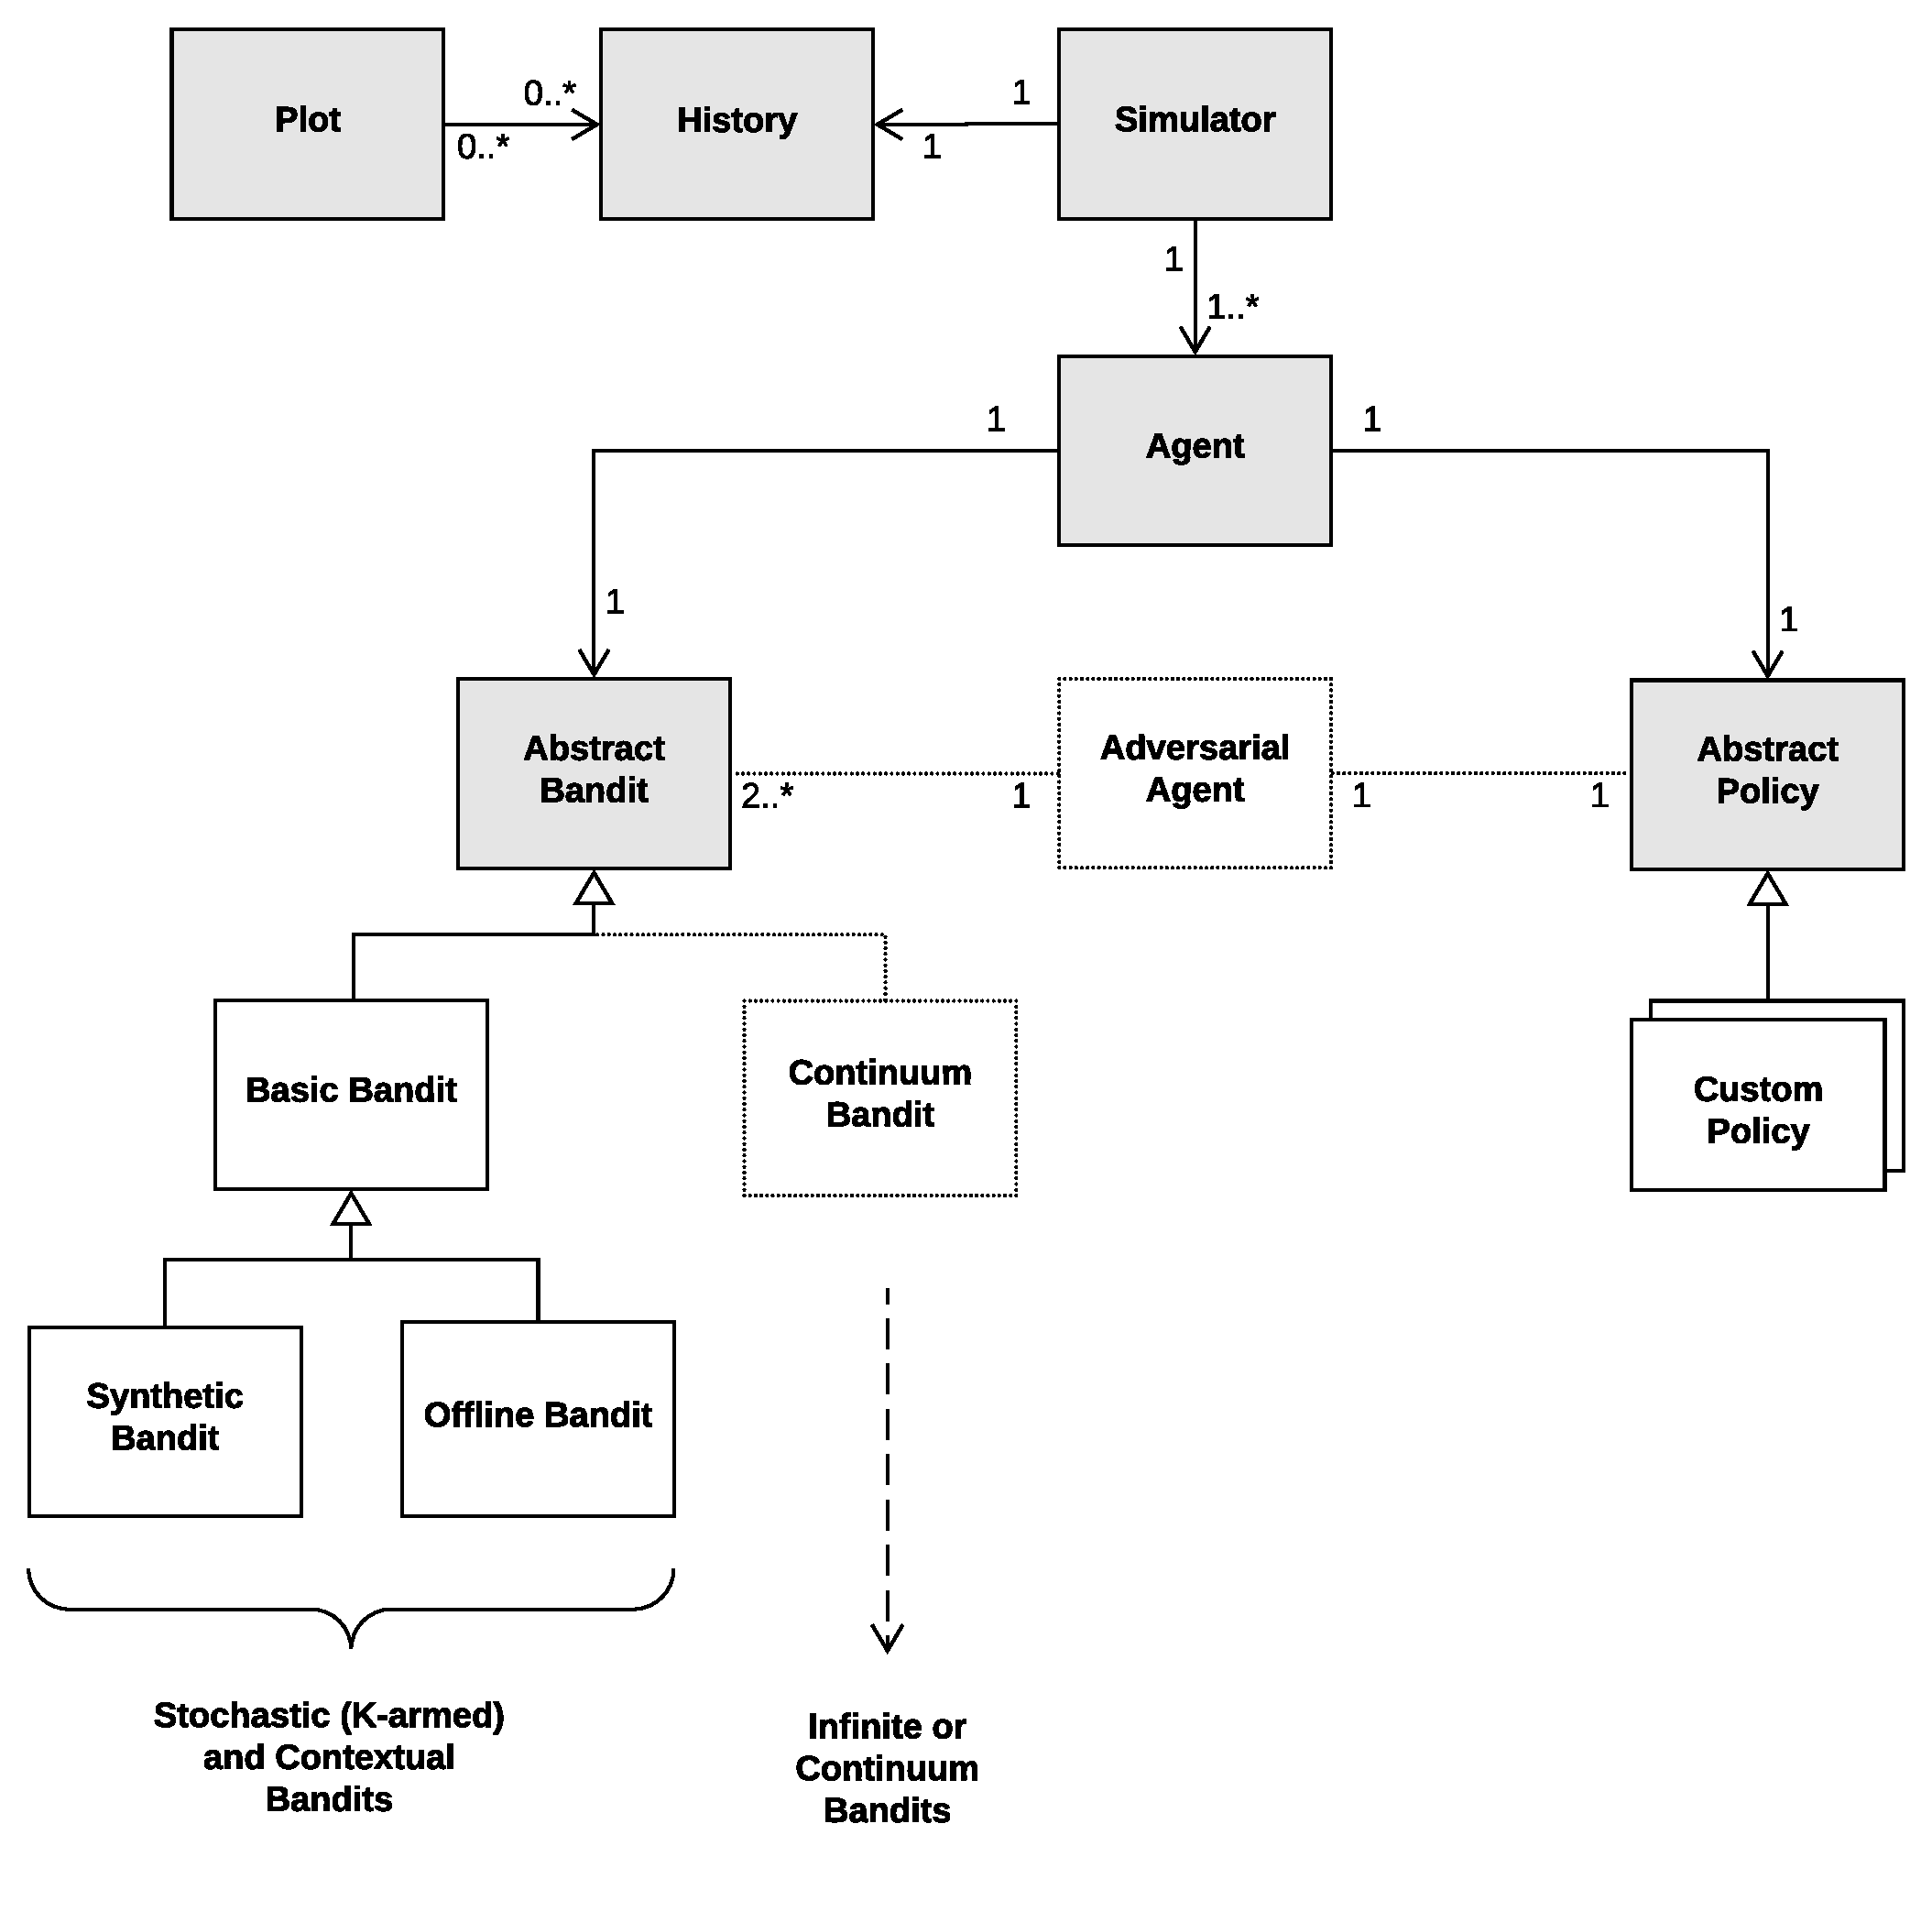
\includegraphics[width=.99\textwidth]{fig/contextual_class}
    \label{fig:contextual_class}
      \caption{\pkg{contextual} UML Class Diagram}
\end{figure}

\begin{figure}[H]
  \centering
    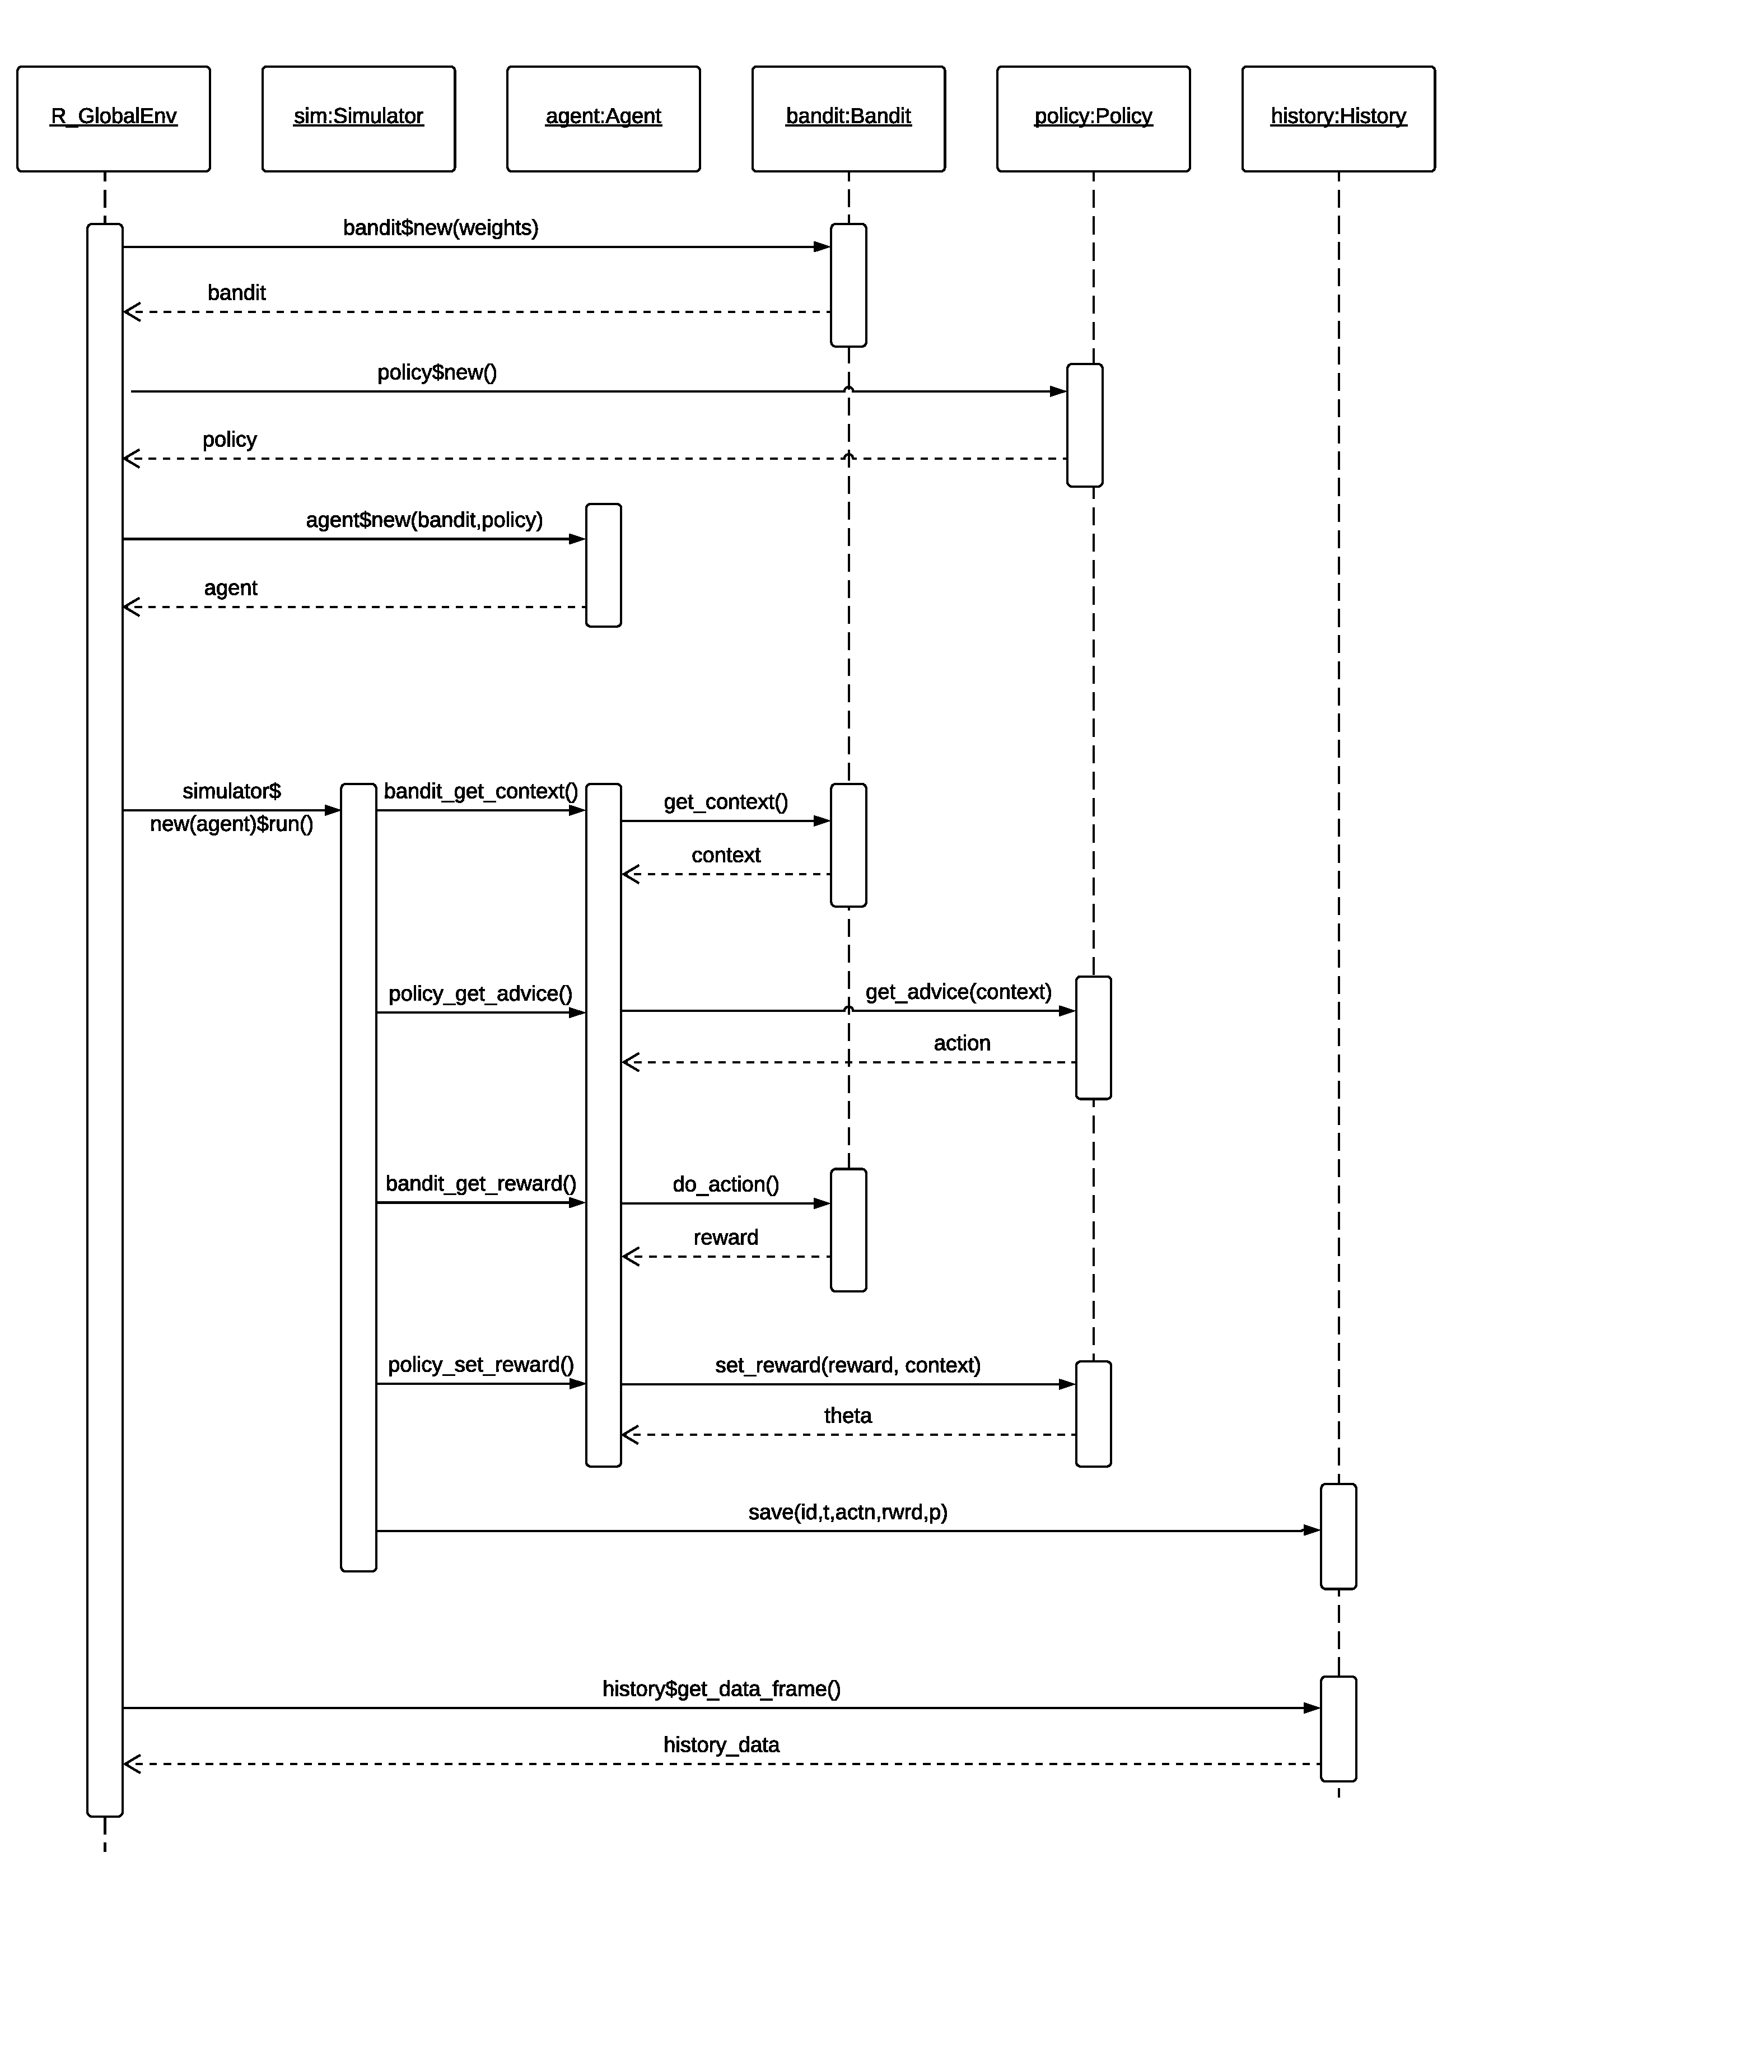
\includegraphics[width=.99\textwidth]{fig/contextual_sequence}
    \label{fig:contextual_sequence}
      \caption{\pkg{contextual} UML Sequence Diagram}
\end{figure}

\section{Special features}
%% Note: If there is markup in \(sub)section, then it has to be escape as above.

For instance, quantifying variance..

\section{The art of optimal parallelisation}
%% Note: If there is markup in \(sub)section, then it has to be escape as above.

There is a very intersting trade of between the amount of parallelisation (how many cores, nodes used) the resources needed to compute a certain model, and the amount of data going to and fro the cores.

PERFORMANCE DATA  ------------------------------------------------------------

on 58  cores:    k3*d3 * 5 policies * 300  * 10000 --\textgreater{} 132 seconds

on 120 cores:    k3*d3 * 5 policies * 300  * 10000 --\textgreater{} 390 seconds

---

on 58  cores:    k3*d3 * 5 policies * 3000 * 10000 --\textgreater{} 930 seconds

on 120 cores:    k3*d3 * 5 policies * 3000 * 10000 --\textgreater{} 691 seconds



\section{Extra greedy UCB}
%% Note: If there is markup in \(sub)section, then it has to be escape as above.

Ladila bladibla.

\section{Conclusions}
\label{sec:conc4}


Placeholder... the goal of a data analysis is not only to answer a research question based on data but also to collect findings that support that answer. These findings usually take the form of a~table, plot or regression/classification model and are usually presented in articles or reports.

\section{Acknowledgments}

Thanks go to CCC.

%\bibliographystyle{apacite}
\bibliography{jss}

\end{document}
